\documentclass[aspectratio=169, 10pt]{beamer}
\usepackage{fontspec}
\setmainfont{Times New Roman}

\usepackage{amsmath,amssymb,amsfonts}
\usepackage{graphicx}
\usepackage{booktabs}
\usepackage{tabularx}
\usepackage{xcolor}

\usetheme{Boadilla}
\usecolortheme{whale}

% Bỏ hiệu ứng đổ bóng của tất cả slide
\setbeamertemplate{blocks}[rounded][shadow=false]

% Bỏ thanh điều hướng beamer
\setbeamertemplate{navigation symbols}{}

% Bỏ môn học và người thuyết trình ở footer, chỉ để lại số thứ tự trang
\setbeamertemplate{footline}{
    \leavevmode%
    \hbox{%
    \begin{beamercolorbox}[wd=\paperwidth,ht=2.5ex,dp=1.1ex,right]{page number in head/foot}%
        \usebeamerfont{page number in head/foot}\insertframenumber{} / \inserttotalframenumber\hspace*{2.5ex}
    \end{beamercolorbox}}%
    \vskip0pt%
}

% Định nghĩa màu sắc
\definecolor{HUSTRed}{RGB}{186, 12, 47}
\definecolor{NavyBlue}{RGB}{20, 45, 85}
\setbeamercolor{palette primary}{bg=NavyBlue,fg=white}
\setbeamercolor{palette secondary}{bg=NavyBlue!80,fg=white}
\setbeamercolor{palette tertiary}{bg=NavyBlue!60,fg=white}
\setbeamercolor{structure}{fg=NavyBlue}
\setbeamercolor{title}{fg=white,bg=NavyBlue}

% Tiêu đề bìa: Thay suy diễn thống kê thành suy luận thống kê, bỏ subtitle học phần
\title{\textbf{SUY LUẬN THỐNG KÊ TRÊN DỮ LIỆU TẬP LUYỆN GYM}}
\author[Nam Khánh, Thảo]{
    \texorpdfstring{\textbf{Nguyễn Văn Nam Khánh} - 202419069 \\ \textbf{Nguyễn Thị Thảo} - 202419101}{Nguyễn Văn Nam Khánh - 202419069, Nguyễn Thị Thảo - 202419101}
}
\institute{
    Đại học Bách khoa Hà Nội
}
\date{Tháng 11 Năm 2026}

\begin{document}

% Slide 1: Bìa
\begin{frame}[plain]
    \titlepage
\end{frame}

% Slide 2: 1. Tổng quan đề tài và bộ dữ liệu
\begin{frame}{1. Tổng quan đề tài và bộ dữ liệu}
    \begin{columns}
        \begin{column}{0.55\textwidth}
            \textbf{Mục tiêu nghiên cứu}:
            \begin{itemize}
                \item Phân tích các yếu tố ảnh hưởng đến lượng calo tiêu thụ (\texttt{Calories\_Burned}).
                \item Đánh giá tác động của thời lượng tập (\texttt{Session\_Duration}), loại bài tập (\texttt{Workout\_Type}) và giới tính (\texttt{Gender}).
            \end{itemize}
            \vspace{5pt}
            \textbf{Bộ dữ liệu Gym Members Exercise}:
            \begin{itemize}
                \item Quy mô mẫu: $n = 973$ thành viên phòng gym.
                \item Gồm 15 biến (12 định lượng, 3 định tính).
                \item $100\%$ sạch: $0$ giá trị khuyết, $0$ bản ghi trùng.
            \end{itemize}
        \end{column}
        \begin{column}{0.45\textwidth}
            \begin{block}{Phân loại biến trọng tâm}
                \begin{itemize}
                    \item \textbf{Biến phụ thuộc ($Y$)}: \texttt{Calories\_Burned} (kcal).
                    \item \textbf{Biến độc lập ($x$)}: \texttt{Session\_Duration} (giờ).
                    \item \textbf{Biến phân loại}: \texttt{Gender}, \texttt{Workout\_Type}, \texttt{Experience\_Level}.
                    \item \textbf{Biến sinh lý}: \texttt{Avg\_BPM}, \texttt{Max\_BPM}, \texttt{Weight}, \texttt{BMI}.
                \end{itemize}
            \end{block}
        \end{column}
    \end{columns}
\end{frame}

% Slide 3: 2. Chương 1: mẫu ngẫu nhiên và cơ sở toán học
\begin{frame}{2. Chương 1: mẫu ngẫu nhiên và cơ sở toán học}
    \begin{block}{Cơ sở lý thuyết mẫu ngẫu nhiên và thống kê mẫu}
        \footnotesize
        \begin{itemize}\setlength\itemsep{1pt}
            \item \textbf{Mẫu ngẫu nhiên}: $W_X = (X_1, X_2, \dots, X_n)$ kích thước $n$ gồm các biến ngẫu nhiên độc lập có cùng phân phối xác suất với biến ngẫu nhiên gốc $X$. Mẫu cụ thể: $W_x = (x_1, x_2, \dots, x_n)$.
            \item \textbf{Trung bình mẫu}: $\overline{X} = \frac{1}{n}\sum_{i=1}^n X_i$, có $E(\overline{X}) = \mu$ (ước lượng không chệch) và $V(\overline{X}) = \frac{\sigma^2}{n}$. Giá trị quan sát: $\overline{x} = \frac{1}{n}\sum_{i=1}^n x_i$.
            \item \textbf{Phương sai mẫu và phương sai mẫu hiệu chỉnh}:
            \[ \widetilde{S}^2 = \frac{1}{n}\sum_{i=1}^n (X_i - \overline{X})^2 \quad \longrightarrow \quad S^2 = \frac{n}{n-1}\widetilde{S}^2 = \frac{1}{n-1}\sum_{i=1}^n (X_i - \overline{X})^2 \]
            Ta có $E(\widetilde{S}^2) = \frac{n-1}{n}\sigma^2$ (ước lượng chệch), trong khi $E(S^2) = \sigma^2$ (ước lượng không chệch).
            \item \textbf{Tần suất mẫu}: $\widehat{P} = \frac{Y}{n}$ (với $Y \sim B(n, p)$), $E(\widehat{P}) = p, V(\widehat{P}) = \frac{p(1-p)}{n}$. Giá trị quan sát: $f = k/n$.
        \end{itemize}
    \end{block}
    \vspace{2pt}
    \footnotesize\textbf{Phân phối mẫu}: Khi kích thước mẫu lớn ($n = 973 \ge 30$), theo Định lý giới hạn trung tâm, thống kê $Z = \frac{\overline{X} - \mu}{S/\sqrt{n}} \xrightarrow{d} N(0, 1)$, thống kê $T = \frac{\overline{X} - \mu}{S/\sqrt{n}} \sim t(n-1)$, và $\frac{(n-1)S^2}{\sigma^2} \sim \chi^2(n-1)$.
\end{frame}

% Slide 4: 3. Thống kê mô tả thực nghiệm ($n = 973$)
\begin{frame}{3. Thống kê mô tả thực nghiệm ($n = 973$)}
    \begin{table}[H]
    \centering\footnotesize
    \begin{tabular}{lrrrrrr}
    \toprule
    \textbf{Biến số} & \textbf{Trung bình ($\bar{x}$)} & \textbf{Độ lệch chuẩn ($s$)} & \textbf{Trung vị} & \textbf{Min} & \textbf{Max} \\
    \midrule
    \texttt{Calories\_Burned} (kcal) & 905.42 & 272.64 & 893.00 & 285.00 & 1650.00 \\
    \texttt{Session\_Duration} (giờ) & 1.256 & 0.343 & 1.25 & 0.50 & 2.00 \\
    \texttt{Avg\_BPM} (nhịp/phút) & 143.44 & 15.23 & 143.00 & 120.00 & 170.00 \\
    \texttt{Weight} (kg) & 73.09 & 15.00 & 72.80 & 40.00 & 115.00 \\
    \midrule
    \texttt{Gender = Male} & \multicolumn{5}{c}{$k = 511$, $f = 52.52\%$} \\
    \texttt{Workout\_Type: Cardio} & \multicolumn{5}{c}{$k = 251$, $f = 25.80\%$} \\
    \texttt{Workout\_Type: HIIT} & \multicolumn{5}{c}{$k = 247$, $f = 25.39\%$} \\
    \bottomrule
    \end{tabular}
    \end{table}
    \textit{Toàn bộ các hàm thống kê được nhóm tự cài đặt trong mô-đun \texttt{src/stats\_utils.py}.}
\end{frame}

% Slide 5: 4. Chương 2: ước lượng điểm và khoảng tin cậy 95%
\begin{frame}{4. Chương 2: ước lượng điểm và khoảng tin cậy 95\%}
    \begin{columns}
        \begin{column}{0.5\textwidth}
            \textbf{Phương pháp ước lượng điểm}:
            \begin{itemize}
                \item \textbf{Phương pháp mô men và hợp lý cực đại} cho $\mu$: $\hat{\mu} = \bar{x} = 905.42$ kcal.
                \item \textbf{Phương pháp hợp lý cực đại} cho $\sigma^2$: $\hat{\sigma}^2 = \frac{1}{n}\sum (x_i - \bar{x})^2$ (chệch dưới). Nhân $\frac{n}{n-1}$ thu được $s^2 = 0.1177$ (hiệu chỉnh không chệch).
            \end{itemize}
            \vspace{5pt}
            \textbf{Diễn giải tần suất độ tin cậy 95\%}:
            \begin{quote}
                \small ``Nếu lặp lại việc lấy mẫu độc lập 973 người vô hạn lần, thì 95\% các khoảng tin cậy tính được sẽ chứa đúng tham số thực của tổng thể.''
            \end{quote}
        \end{column}
        \begin{column}{0.5\textwidth}
            \begin{block}{Kết quả khoảng tin cậy 95\% hai phía}
                \footnotesize
                \begin{itemize}
                    \item $\mu_{\text{Calories}}$: $[888.27, 922.57]$ (phân phối Student $t$, bậc tự do $972$).
                    \item $\sigma^2_{\text{Duration}}$: $[0.1079, 0.1289]$ (phân phối $\chi^2$, bậc tự do $972$).
                    \item $\sigma_{\text{Duration}}$: $[0.3284, 0.3590]$ (căn bậc hai khoảng tin cậy $\sigma^2$).
                    \item $p_{\text{Male}}$: $[0.4938, 0.5566]$ (xấp xỉ phân phối chuẩn tắc $Z$).
                    \item $\mu_1 - \mu_2$ (Nam -- Nữ): $[48.47, 115.95]$ (hai phương sai chưa biết, khác nhau).
                    \item $p_1 - p_2$ (Calo $\ge 1000$): $[0.0735, 0.1912]$ (xấp xỉ chuẩn tắc $Z$).
                \end{itemize}
            \end{block}
        \end{column}
    \end{columns}
\end{frame}

% Slide 6: 5. Chương 3: kiểm định tham số và 3 cách tiếp cận
\begin{frame}{5. Chương 3: kiểm định tham số và 3 cách tiếp cận}
    \begin{block}{Quy trình kiểm định và tính nhất quán của 3 cách tiếp cận}
        \footnotesize
        (1) Cặp giả thuyết $H_0/H_1$ $\rightarrow$ (2) Mức ý nghĩa $\alpha = 0.05$ $\rightarrow$ (3) Tiêu chuẩn kiểm định $\rightarrow$ (4) Tính giá trị quan sát, $P$-giá trị $\rightarrow$ (5) Kết luận.
        \begin{itemize}
            \item \textbf{Cách 1 (Miền bác bỏ)}: Giá trị quan sát rơi vào miền bác bỏ $W_\alpha$.
            \item \textbf{Cách 2 ($P$-giá trị)}: $P\text{-giá trị} \le \alpha = 0.05$.
            \item \textbf{Cách 3 (Đối chiếu khoảng tin cậy)}: Giá trị giả định $\theta_0$ không thuộc khoảng tin cậy 95\% tương ứng.
        \end{itemize}
    \end{block}

    \begin{table}[H]
    \centering\scriptsize
    \begin{tabular}{@{}lcccc@{}}
    \toprule
    \textbf{Kiểm định} & \textbf{Giả thuyết $H_0$} & \textbf{Thống kê quan sát} & \textbf{$P$-giá trị} & \textbf{Kết luận ($\alpha = 0.05$)} \\
    \midrule
    Kỳ vọng Calo & $\mu = 900$ & $t_0 = 0.620$ & 0.5352 & Không bác bỏ $H_0$ \\
    Phương sai Thời lượng & $\sigma^2 = 0.10$ & $k_0^2 = 1143.77$ & 0.0002 & \textbf{Bác bỏ $H_0$} \\
    Tỷ lệ Nam giới & $p = 0.50$ & $z_0 = 1.571$ & 0.1162 & Không bác bỏ $H_0$ \\
    So sánh 2 phương sai Calo & $\sigma_1^2 = \sigma_2^2$ & $f_0 = 1.318$ & 0.0025 & \textbf{Bác bỏ $H_0$} ($\sigma_1^2 \ne \sigma_2^2$) \\
    So sánh 2 kỳ vọng Calo & $\mu_1 = \mu_2$ & $t_0 = 4.781$ & $2.01 \times 10^{-6}$ & \textbf{Bác bỏ $H_0$} (Nam đốt calo cao hơn) \\
    \bottomrule
    \end{tabular}
    \end{table}
\end{frame}

% Slide 7: 6. Chương 3: phân tích phương sai một nhân tố và phi tham số
\begin{frame}{6. Chương 3: phân tích phương sai một nhân tố và phi tham số}
    \begin{columns}
        \begin{column}{0.5\textwidth}
            \textbf{Phân tích phương sai một nhân tố}:
            \[ H_0: \mu_{\text{Cardio}} = \mu_{\text{HIIT}} = \mu_{\text{Strength}} = \mu_{\text{Yoga}} \]
            \begin{table}[H]
            \centering\scriptsize
            \begin{tabular}{lrrrr}
            \toprule
            \textbf{Nguồn biến thiên} & \textbf{SS} & \textbf{Bậc tự do} & \textbf{MS} & \textbf{Thống kê $F_0$} \\
            \midrule
            Nhân tố (giữa các nhóm) & $1.48 \times 10^6$ & 3 & 493,760 & \textbf{6.7644} \\
            Sai số (trong nội bộ) & $7.08 \times 10^7$ & 969 & 73,035 & -- \\
            \bottomrule
            \end{tabular}
            \end{table}
            $F_0 = 6.7644 > f_{0.05; 3; 969} = 2.6141$ ($P\text{-giá trị} = 0.00016$).
            $\rightarrow$ \textbf{Bác bỏ $H_0$}: Loại bài tập có ảnh hưởng thực sự đến lượng calo tiêu thụ.
        \end{column}
        \begin{column}{0.5\textwidth}
            \textbf{Kiểm định phi tham số Chi-bình phương}:
            \begin{itemize}
                \item \textbf{Sự phù hợp của phân phối xác suất (chuẩn)}:
                \begin{itemize}
                    \item \texttt{Session\_Duration}: $k_0^2 = 2.4578, P = 0.9303 > 0.05$.
                    \item \texttt{Calories\_Burned}: $k_0^2 = 5.2140, P = 0.6338 > 0.05$.
                    \item $\rightarrow$ Phù hợp với phân phối chuẩn!
                \end{itemize}
                \item \textbf{Kiểm định tính độc lập}:
                \begin{itemize}
                    \item Bảng tiếp biến $2 \times 3$, bậc tự do $(2-1)(3-1) = 2$.
                    \item $k_0^2 = 0.0128 < \chi^2_{0.05; 2} = 5.9915$ ($P = 0.9936$).
                    \item $\rightarrow$ Không bác bỏ $H_0$: Giới tính và cấp độ kinh nghiệm độc lập nhau!
                \end{itemize}
            \end{itemize}
        \end{column}
    \end{columns}
\end{frame}

% Slide 8: 7. Chương 4.1: hồi quy tuyến tính đơn
\begin{frame}{7. Chương 4.1: hồi quy tuyến tính đơn}
    \begin{columns}
        \begin{column}{0.5\textwidth}
            \textbf{Mô hình hồi quy tuyến tính đơn}:
            \[ Y = \beta_0 + \beta_1 x + \varepsilon, \quad \varepsilon \sim N(0, \sigma^2) \]
            \footnotesize
            \begin{itemize}\setlength\itemsep{1.5pt}
                \item Phương trình hồi quy mẫu (bình phương bé nhất):
                \[ \hat{y} = -1.4465 + 721.7860 \cdot x \]
                \item Hệ số xác định $R^2 = 0.8247$: Thời lượng tập giải thích $82.47\%$ biến thiên lượng calo.
                \item Hệ số góc $\hat{\beta}_1 = 721.79$ ($P\text{-giá trị} < 10^{-15}$): Mỗi giờ tập tăng đốt thêm 721.8 kcal.
            \end{itemize}
            \begin{block}{Mối liên hệ giữa kiểm định $T_0$ và $F_0$}
                \scriptsize
                \[ T_0^2 = \left(\frac{\hat{\beta}_1}{s / \sqrt{S_{xx}}}\right)^2 = \frac{\hat{\beta}_1^2 S_{xx}}{s^2} = \frac{MSR}{MSE} = F_0 \]
                Thực nghiệm: $T_0^2 = 67.5920^2 = 4568.6744 = F_0$.
            \end{block}
        \end{column}
        \begin{column}{0.5\textwidth}
            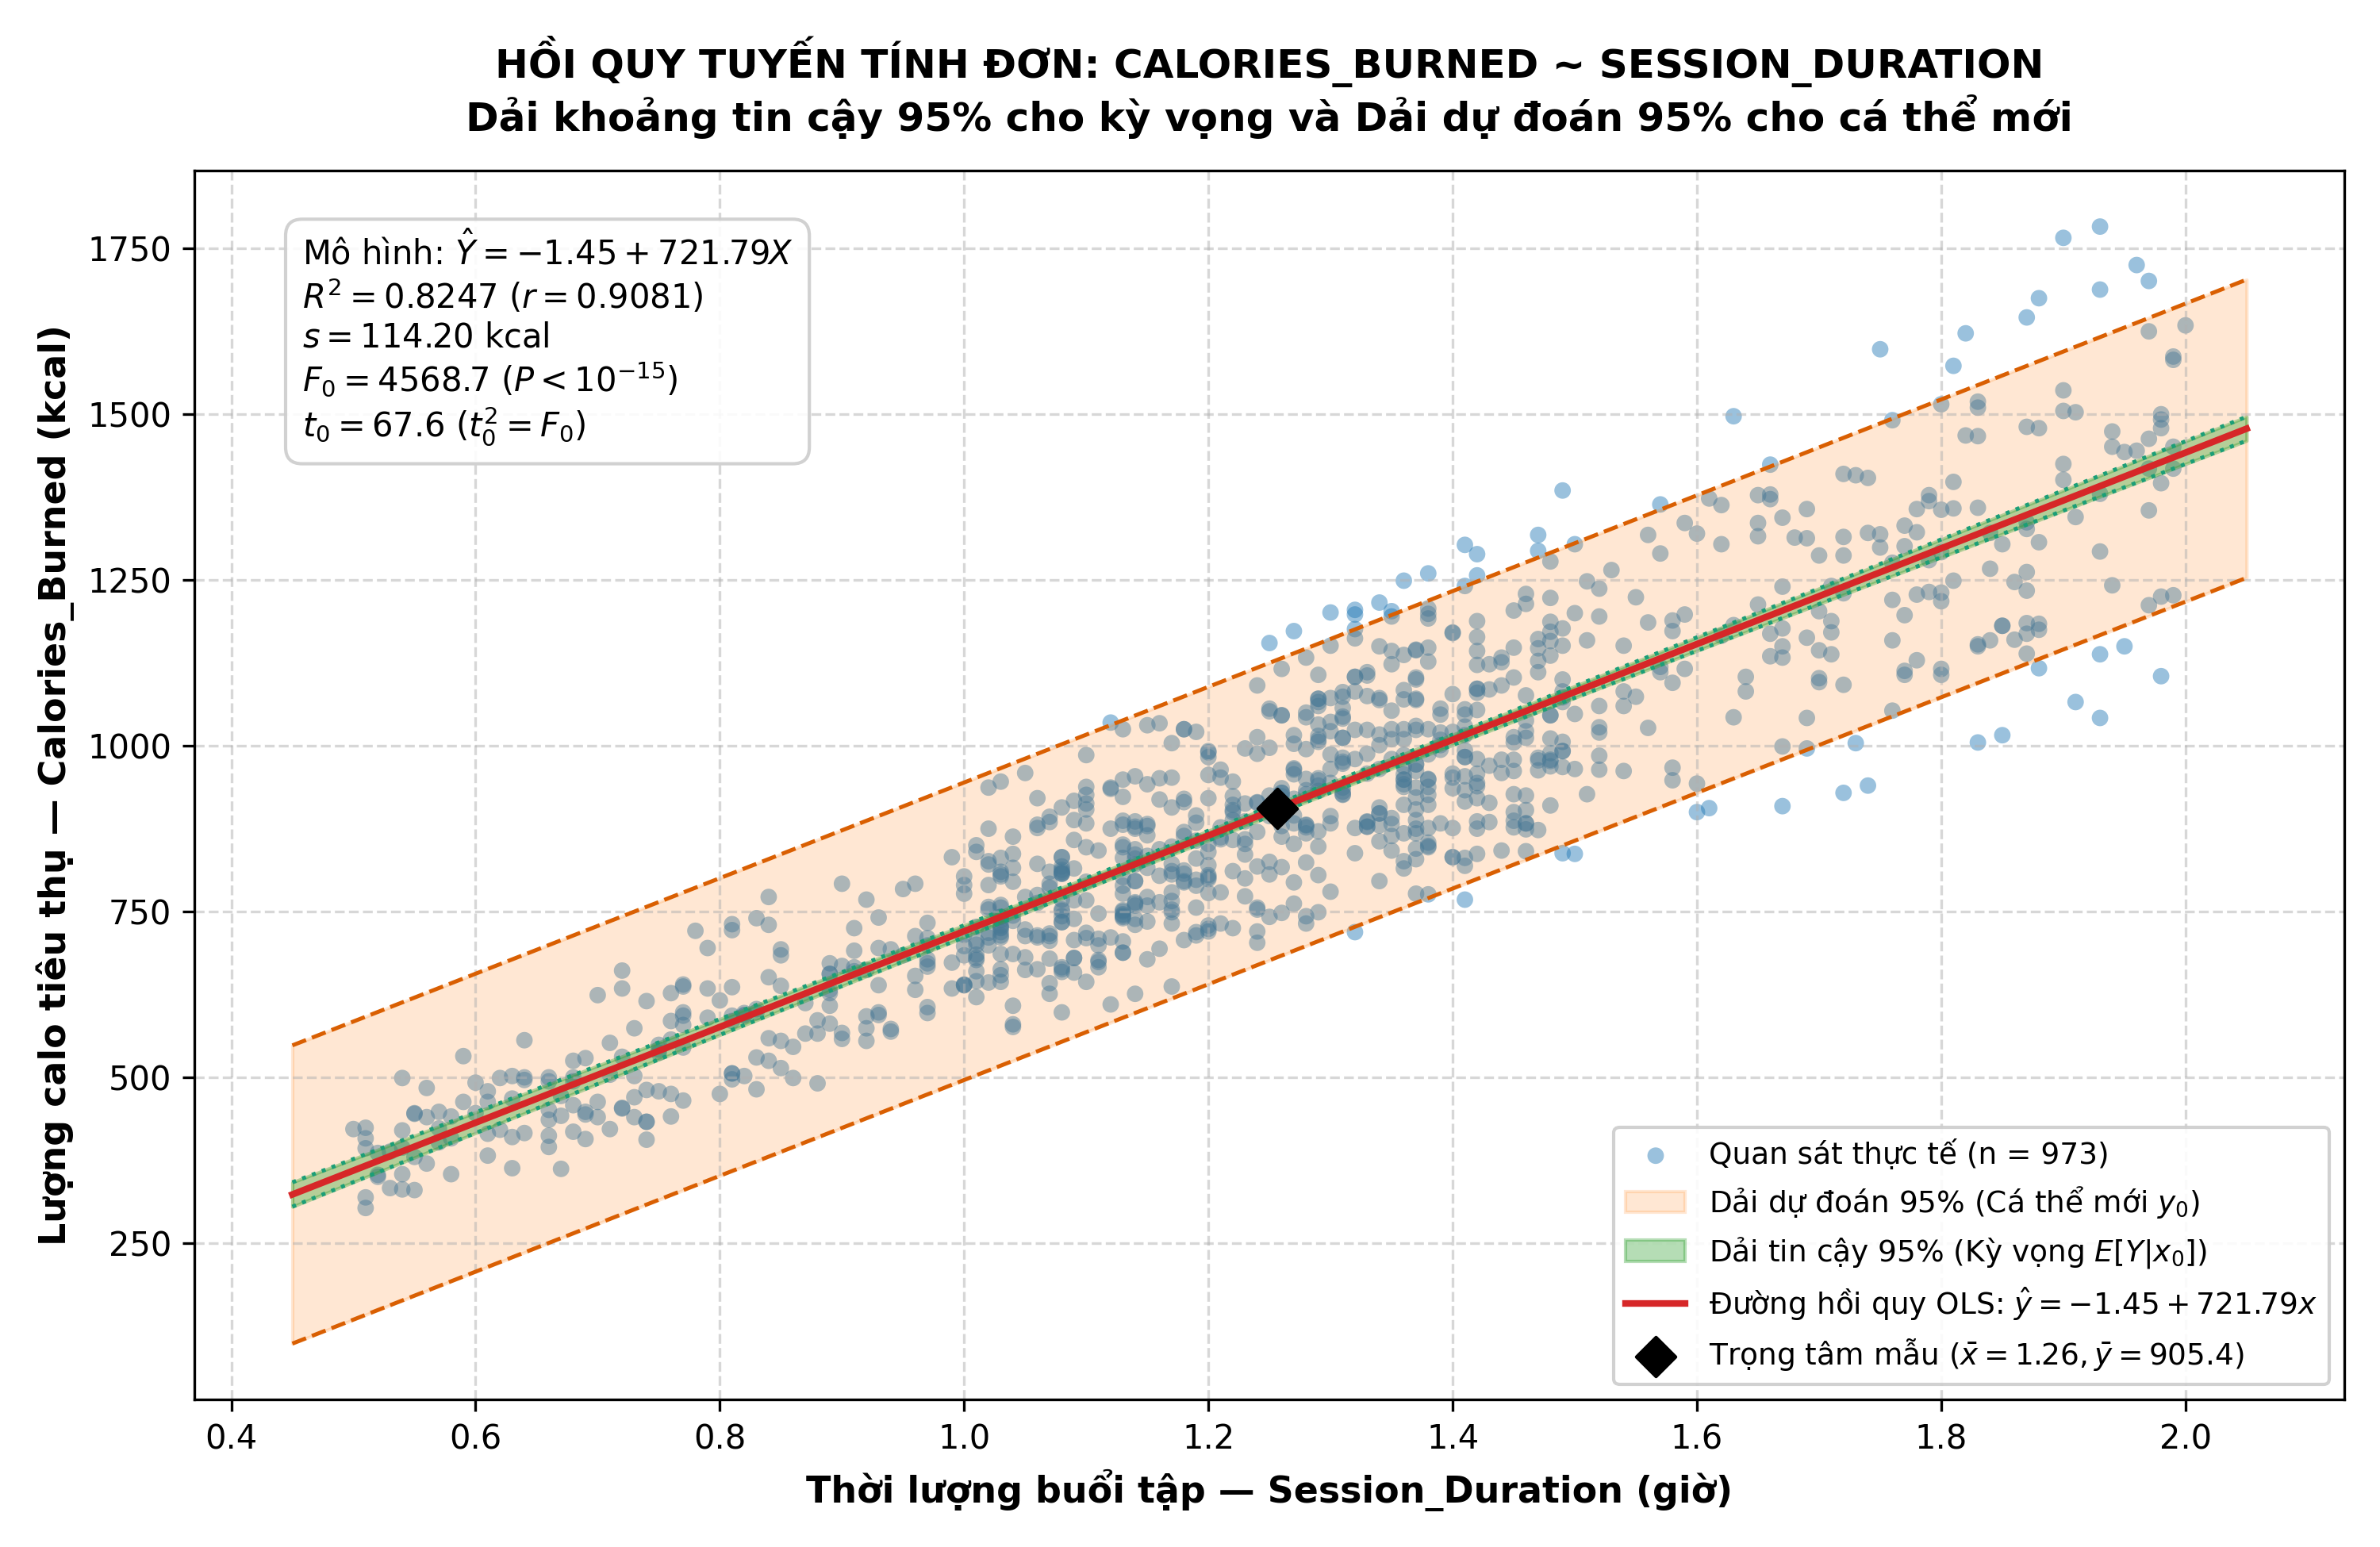
\includegraphics[width=\textwidth]{../outputs/figures/05_slr_bands.png}
        \end{column}
    \end{columns}
\end{frame}

% Slide 9: 8. Khoảng tin cậy so với khoảng dự đoán và ý nghĩa hệ số chặn
\begin{frame}{8. Khoảng tin cậy so với khoảng dự đoán và ý nghĩa hệ số chặn}
    \begin{columns}
        \begin{column}{0.5\textwidth}
            \textbf{So sánh dải khoảng tin cậy và dải dự đoán}:
            \begin{itemize}
                \item \textbf{Khoảng tin cậy cho $E(Y|x_0)$}: Ước lượng kỳ vọng tổng thể.
                \[ \hat{y}_0 \pm t_{\alpha/2}(n-2) \cdot s \sqrt{\frac{1}{n} + \frac{(x_0 - \bar{x})^2}{S_{xx}}} \]
                \item \textbf{Khoảng dự đoán cho cá thể mới $y_0$}:
                \[ \hat{y}_0 \pm t_{\alpha/2}(n-2) \cdot s \sqrt{\mathbf{1} + \frac{1}{n} + \frac{(x_0 - \bar{x})^2}{S_{xx}}} \]
                \item \textit{Tại sao luôn rộng hơn?} Vì chứa thêm số hạng ``$+1$'', biểu diễn phương sai sai số tự nhiên của cá thể mới: $V(y_0 - \hat{y}_0) = V(\hat{y}_0) + \sigma^2$.
            \end{itemize}
        \end{column}
        \begin{column}{0.5\textwidth}
            \begin{block}{Ý nghĩa thực tế và toán học của hệ số chặn $\hat{\beta}_0 = -1.45$}
                \begin{itemize}
                    \item \textbf{Về thực tế}: Dữ liệu không có buổi tập nào $0$ giờ ($x \in [0.5, 2.0]$). Ngoại suy tại $x=0$ không mang ý nghĩa thực tiễn.
                    \item \textbf{Về toán học}: $\hat{\beta}_0$ là mỏ neo toán học bắt buộc để:
                    \begin{enumerate}
                        \item Đảm bảo tổng phần dư $\sum e_i = 0$.
                        \item Buộc đường hồi quy đi qua trọng tâm $(\bar{x}, \bar{y})$.
                        \item Giữ phân rã tổng bình phương $SST = SSR + SSE$.
                    \end{enumerate}
                \end{itemize}
            \end{block}
        \end{column}
    \end{columns}
\end{frame}

% Slide 10: 9. Chương 4.2: phân tích phần dư và hệ số tương quan
\begin{frame}{9. Chương 4.2: phân tích phần dư và hệ số tương quan}
    \begin{columns}
        \begin{column}{0.5\textwidth}
            \textbf{Chẩn đoán phần dư ($e_i = y_i - \hat{y}_i$)}:
            \begin{itemize}
                \item Kỳ vọng sai số $E(e_i) \approx 0$, hệ số bất đối xứng $-0.02$, hệ số nhọn $0.05$.
                \item Phương sai sai số đồng nhất (thuần nhất).
                \item Đồ thị xác suất bám sát đường phân phối chuẩn.
            \end{itemize}
            \vspace{5pt}
            \textbf{Hệ số tương quan mẫu $r = 0.9081$}:
            \begin{itemize}
                \item Kiểm định $H_0: \rho = 0$: $t_0 = 67.592$ ($P\text{-giá trị} < 10^{-15}$).
                \item Biến đổi Fisher: $U = \frac{1}{2}\ln \frac{1+r}{1-r} = \text{arctanh}(r) = 1.5167$.
                \item Kiểm định $H_0: \rho = 0.85$: $Z_0 = \frac{U - U_0}{\sqrt{1/(n-3)}} = 8.1633 \rightarrow$ Bác bỏ.
                \item Khoảng tin cậy 95\% cho hệ số tương quan $\rho$: $[0.8965, 0.9185]$.
            \end{itemize}
        \end{column}
        \begin{column}{0.5\textwidth}
            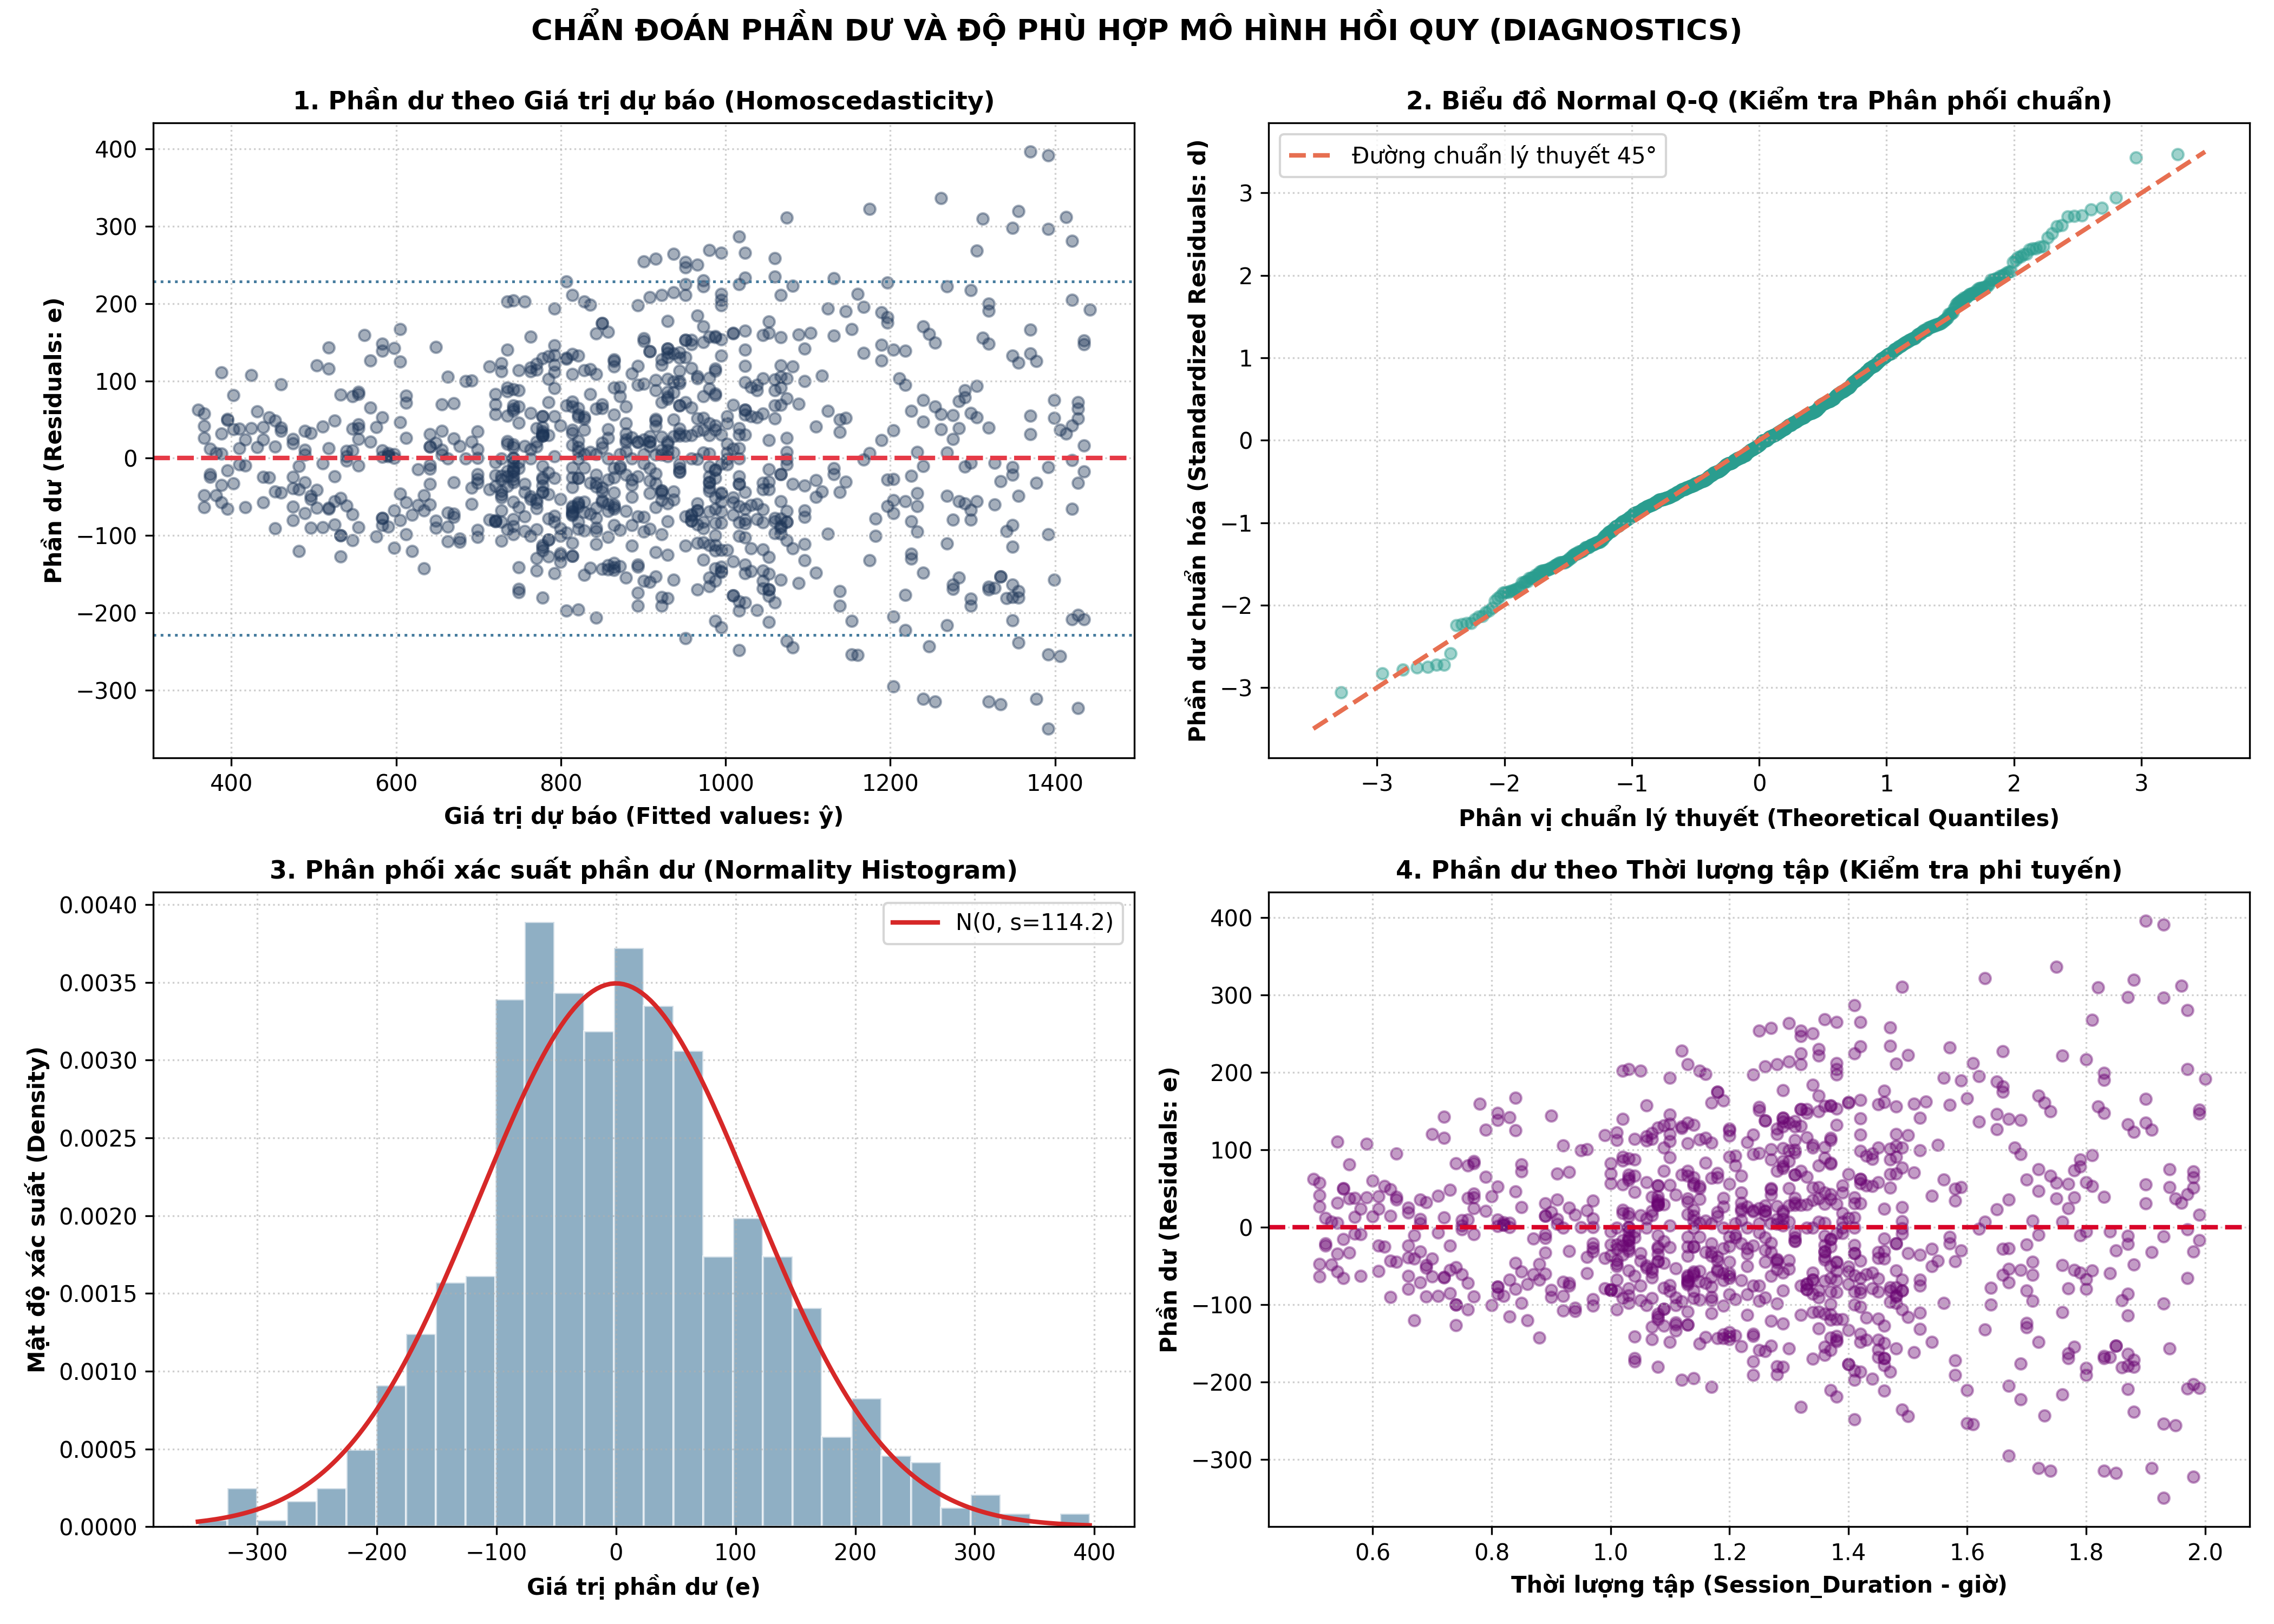
\includegraphics[width=\textwidth]{../outputs/figures/06_residual_diagnostics.png}
        \end{column}
    \end{columns}
\end{frame}

% Slide 11: 10. Trả lời câu hỏi trọng tâm: tương quan và nhân quả
\begin{frame}{10. Trả lời câu hỏi trọng tâm: tương quan và nhân quả}
    \begin{block}{Nguyên lý cốt lõi: ``Tương quan không đồng nghĩa với nhân quả''}
        Mặc dù hệ số $r = 0.9081$ rất cao, \textbf{thời lượng tập không phải nguyên nhân duy nhất} quyết định lượng calo tiêu thụ!
    \end{block}
    \vspace{5pt}
    \textbf{Các yếu tố cùng chi phối}:
    \begin{enumerate}
        \item \textbf{Cường độ gắng sức tim mạch (\texttt{Avg\_BPM}, \texttt{Max\_BPM})}: Người tập ở nhịp tim $160$ BPM tiêu thụ calo vượt trội so với nhịp tim $110$ BPM trong cùng thời gian tập.
        \item \textbf{Khối lượng cơ thể (\texttt{Weight})}: Thể trọng lớn đòi hỏi tiêu hao công năng cơ học lớn hơn.
        \item \textbf{Loại bài tập (\texttt{Workout\_Type})}: HIIT và Cardio đốt cháy calo trên mỗi phút tập cao hơn nhiều so với Yoga.
    \end{enumerate}
    \vspace{3pt}
    $\longrightarrow$ \textbf{Định hướng phát triển}: Mở rộng sang mô hình \textbf{Hồi quy tuyến tính bội} để kiểm soát đồng thời tác động của nhiều biến giải thích.
\end{frame}

% Slide 12: 11. Tổng kết
\begin{frame}{11. Tổng kết}
    \begin{columns}
        \begin{column}{0.5\textwidth}
            \textbf{Sản phẩm hoàn thành}:
            \begin{itemize}
                \item \texttt{main.py}: Chạy tuần tự 6 mô-đun và kiểm tra chéo tự động trong $25$ giây.
                \item Báo cáo toàn văn: \texttt{BaoCao\_SLTK\_Nhom18.pdf}.
                \item Slide thuyết trình Beamer: \texttt{Slide\_ThuyetTrinh\_Nhom18.pdf}.
                \item Mã nguồn và tài liệu lưu trữ đầy đủ trong thư mục dự án.
            \end{itemize}
        \end{column}
        \begin{column}{0.5\textwidth}
            \textbf{Kết quả thực nghiệm chính}:
            \begin{itemize}
                \item \textbf{Mẫu và ước lượng}: Kích thước $n=973$; ước lượng điểm và khoảng tin cậy 95\% vững chắc cho kỳ vọng, phương sai, tỷ lệ.
                \item \textbf{Kiểm định và phân tích phương sai}: Bác bỏ tính đồng nhất calo theo loại bài tập ($F_0 = 6.7644$, $P < 0.001$).
                \item \textbf{Hồi quy và tương quan}: $R^2 = 82.47\%$, hệ số tương quan mẫu $r = 0.9081$, mở rộng sang hồi quy tuyến tính bội.
            \end{itemize}
        \end{column}
    \end{columns}
\end{frame}

% Slide 13: 12. Thank you
\begin{frame}[c]{12. Thank you}
    \begin{center}
        \vspace{1.5cm}
        {\Huge\bfseries\color{NavyBlue} THANK YOU!}
        
        \vspace{1cm}
        {\large Cảm ơn thầy cô và các bạn đã chú ý lắng nghe!}
    \end{center}
\end{frame}

\end{document}
